\documentclass{beamer}

\mode<presentation>
{\usetheme{boxes}}

\usepackage{array}
\usepackage{times}
\usepackage{graphicx}
\usepackage{hyperref}
\usepackage{listings}
\usepackage{relsize}
\usepackage{ragged2e}
\usepackage[T1]{fontenc}

\lstdefinestyle{customc}{
  belowcaptionskip=1\baselineskip,
  breaklines=true,
  frame=L,
  xleftmargin=\parindent,
  language=C,
  showstringspaces=false,
  basicstyle=\footnotesize\ttfamily,
  keywordstyle=\bfseries\color{green!40!black},
  commentstyle=\itshape\color{purple!40!black},
  identifierstyle=\color{blue},
  stringstyle=\color{red},
}
\lstdefinestyle{custombash}{
  belowcaptionskip=1\baselineskip,
  breaklines=true,
  frame=L,
  xleftmargin=\parindent,
  language=bash,
  basicstyle=\footnotesize\ttfamily,
  showstringspaces=false,
  commentstyle=\itshape\color{purple!40!black},
  keywordstyle=\itshape\color{green!40!black},
  identifierstyle=\color{blue},
  stringstyle=\color{orange},
}

\usebackgroundtemplate
{
  \hbox to \paperwidth{\hfil
\includegraphics[width=4in,
      height=\paperheight]{wildcat_transparent.jpg}\hfil}
}

\title{PHYS 105 Lecture 5: Strings and Arrays}
\author{Tom McClintock \\
	Dept. of Physics\\
	University of Arizona
}
\date{\today}

\begin{document}

\begin{frame}
  \titlepage
\end{frame}

\begin{frame}
  \frametitle{Last time}
  \begin{itemize}
    \item Binary
    \item More types
    \item Using sizeof()
    \item For loops
  \end{itemize}
\end{frame}

\begin{frame}
  \frametitle{This time}
  \begin{itemize}
    \item Character strings
    \item Arrays
  \end{itemize}
\end{frame}

\begin{frame}
  \frametitle{Character Strings}
  Last time, one of the data types we learned about was \textbf{char}\\
  This type is used to store a character.\\
  How would we store a whole word? It would be a hassle to have a \textbf{char}
  variable for each letter in a word or phrase.\\
  The solution is \textbf{character strings}.
\end{frame}

\begin{frame}[fragile]
  \frametitle{Character Strings}
  \textbf{Character strings} are a single variable that holds many characters.\\
  \begin{lstlisting}[style=customc]
    char *my_string = ``look, I am a string!'';
  \end{lstlisting}
  Then, if we were to print the \textbf{string} with \%s
  \begin{lstlisting}[style=customc]
    printf(``%s \n'', my_string);
  \end{lstlisting}
  the string would be printed back to us on screen.
\end{frame}

\begin{frame}[fragile]
  \frametitle{Character Strings}
  The declaration of the string in the previous slide is done if you
  know what is in the string ahead of time.\\
  Here is another way to declare a string.
  \begin{lstlisting}[style=customc]
    char my_string[20];
  \end{lstlisting}
  Using this method, you give a limit to how long the string will be.\\
  In this example, ``my\_string'' will be at most 20 characters long.
\end{frame}

\begin{frame}[fragile]
  \frametitle{Hello [user]!}
  Here is an example of how one can take a string from the user.\\
  Write it yourself and demonstrate that the computer can print strings back to you.
  \lstinputlisting[style=customc]{string_test.c}
\end{frame}

\begin{frame}
  \frametitle{Arrays}
  Another name for a character string is a character \textbf{array}.\\
  An \textbf{array}, in general, is just a list of items of whatever type you want.\\
  Imagine that instead of having a list of characters (e.g. a word) you had a big list
  of numbers. Again, it would be a hassle to have a variable for each number. This is where
  \textbf{arrays} come in handy.
\end{frame}

\begin{frame}[fragile]
  \frametitle{Declaring Arrays}
  Arrays can be declared in one of two ways, depending on if you know the contents ahead of time:
  \begin{lstlisting}[style=customc]
    int my_array1[] = {2,-3,6,8,55};

    int my_array2[10];
  \end{lstlisting}
  Both of the arrays above are int arrays (a bunch of integers).\\
  ``my\_array1'' has a \textbf{length} of 5 and its elements are already defined.\\
  ``my\_array2'' has a \textbf{length} of 10 and none of its elements are defined. 
  They would have to be defined later on.\\
  Remember that you can have arrays with any kind of data in it including char, int, float, double, etc.
\end{frame}

\begin{frame}[fragile]
  \frametitle{Declaring Arrays}
  When you think of arrays you should have this picture in your mind:
  \begin{center}
    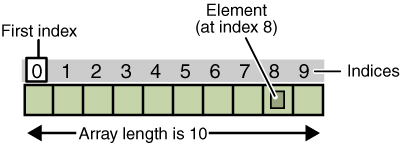
\includegraphics[width=0.5\textwidth]{array_pic.png}
  \end{center}
  A single piece of data in an array is called an \textbf{element} of the array.\\
  Each \textbf{element} is specified by an \textbf{index} of the array.\\
  \vspace{12pt}
  NOTE: Notice that arrays are numbered from 0 to N-1, and have N elements in total.
\end{frame}

\begin{frame}[fragile,allowframebreaks]
  \frametitle{Accessing Array Elements}
  In order to access an \textbf{element} we need to specify an array \textbf{index}.
  This looks like:
  \begin{lstlisting}[style=customc]
    int my_array[10];
   
    my_array[0] = 3;
    my_array[1] = 7;

    my_array[3] = my_array[0];
  \end{lstlisting}
  In this example, the first two elements have been specified as 3 and 7, respectively.\\
  Finally, the fourth element was set equal to the first.
\end{frame}

\begin{frame}[fragile,allowframebreaks]
  \frametitle{letter\_swap.c}
  Try writing this short program that swaps around the first four letters of a string that you enter.
  This is accomplished by exploiting the fact that a string is, in fact, an array.
  \lstinputlisting[style=customc]{letter_swap.c}
\end{frame}

\begin{frame}[fragile]
  \frametitle{Arrays and For Loops}
  Arrays can have many, many elements and it becomes impractical to index them by hand.\\
  For loops are a natural way to \textbf{iterate} over an array to access each element.\\
  In the example below, an array with ten integers is filled in with the numbers 0, 1, 2, ...8, 9.
  \begin{lstlisting}[style=customc]
    int i; // an index

    int my_array[10];
    for( i=0; i<10; i++){
      my_array[i] = i;
    }
  \end{lstlisting}
\end{frame}

\begin{frame}
  \frametitle{Next time}
  \begin{itemize}
    \item Variable operations
    \item While loops
    \item Numerical integration
  \end{itemize}
\end{frame}

\begin{frame}
  \frametitle{In class assignments}
  \begin{enumerate}
    \item Write a program that takes in from the user an integer, n. Then, it declares a \textbf{float} array
      of that many elements. Then, a for loop fills in that array with the numbers 0 up to n, 
      just like in class, and print them out. 
      Show either myself or the TA when you have done this.
    \item Extend the previous program by adding another loop after the first. 
      In this second loop, take a sum of all of the numbers in the array. 
      At the end of the program print out this sum. Demonstrate the series:
      \begin{equation*}
	\sum_{i=0}^{N-1} n_i = \frac{N(N-1)}{2}
      \end{equation*}
  \end{enumerate}
\end{frame}

\begin{frame}
  \frametitle{HW 3 - Quadratic equation due next week}
  A quadratic function has the form:
  \begin{equation*}
    y(x) = ax^2 + bx + c
  \end{equation*}
  This function has two or fewer roots, or locations 
  where it crosses the x-axis.\\
  The equation to find these roots is called the quadratic equation.
  \begin{equation*}
    x_\pm = \frac{-b\pm\sqrt{b^2-4ac}}{2a}
  \end{equation*}
  Take in the coefficients $a$, $b$ and $c$ from the user and use them
  to calculate the roots from the quadratic equation.\\
  Make sure to account for the cases when there are no roots!!
\end{frame}


\end{document}